\documentclass[9pt,aspectratio=169]{beamer}

% --- Theme ---
\usetheme{Singapore}
\setbeamertemplate{navigation symbols}{}   % no icons
\setbeamertemplate{mini frames}{}          % no dots in headline
\setbeamercovered{transparent}

% --- Grayscale colors ---
\definecolor{PelloGrayDark}{RGB}{60,60,60}
\definecolor{PelloGray}{RGB}{120,120,120}
\definecolor{PelloGrayLight}{RGB}{235,235,235}
\definecolor{PelloGrayUltraLight}{RGB}{248,248,248}

\usecolortheme[named=PelloGrayDark]{structure}

% --- Blocks ---
\setbeamertemplate{blocks}[rounded][shadow=false]
\setbeamercolor{block title}{fg=white,bg=PelloGrayDark}
\setbeamercolor{block body}{fg=black,bg=PelloGrayLight}
\setbeamercolor{block title example}{fg=white,bg=PelloGrayDark}
\setbeamercolor{block body example}{fg=black,bg=PelloGrayLight}
\setbeamercolor{section in head/foot}{fg=PelloGray,bg=PelloGrayLight}
\setbeamercolor{subsection in head/foot}{fg=PelloGray,bg=PelloGrayLight}
\setbeamercolor{frametitle}{fg=black}

% --- Itemize bullets (optional; keep if you like the style) ---
\setbeamertemplate{itemize item}{\raisebox{0.2em}{\scalebox{.6}{$\bullet$}}}
\setbeamertemplate{itemize subitem}{\raisebox{0.2em}{\scalebox{1}{$-$}}}

% --- Footer: frame numbers ---
\makeatletter
\setbeamertemplate{footline}{%
  \hfill\usebeamerfont{footline}\insertframenumber/\inserttotalframenumber\hspace{1em}\vspace{2pt}
}
\makeatother

% --- Minimal packages (add more only when needed) ---
\usepackage[english]{babel}
\usepackage[T1]{fontenc}
\usepackage[utf8]{inputenc}
\usepackage{graphicx}
\usepackage{tikz}
\usepackage{booktabs}
\usepackage{makecell} % for jumping lines within cells in tables.
\usepackage{multirow}
\usepackage{amsmath,amssymb,bm}
\usepackage{pifont} % \ding{55} cross mark
\usepackage{hyperref}
\hypersetup{colorlinks,linkcolor=,urlcolor=blue}
\usepackage{comment}
\usepackage{listings}
\lstset{
  language=R,
  basicstyle=\ttfamily\footnotesize,
  keywordstyle=\color{blue},
  commentstyle=\color{green!50!black},
  stringstyle=\color{red},
  frame=single,
  showstringspaces=false
}
\linespread{1.7}   % 1.0 = normal, 1.2–1.5 common
\AtBeginEnvironment{lstlisting}{\linespread{1}\selectfont} % keep code listings single-spaced



% --- Macros ---
\newcommand{\E}{\mathbb{E}}
\newcommand{\Var}{\mathrm{Var}}
\newcommand{\Cov}{\mathrm{Cov}}
\newcommand{\plim}{\operatorname{plim}}
\newcommand{\SEhat}{\widehat{SE}}
\newcommand{\indep}{\perp\!\!\!\perp}
\usetikzlibrary{arrows.meta,positioning}
\tikzset{ % causal diagrams
  -Latex, auto, node distance=1cm and 1.2cm, semithick,
  state/.style={circle, draw=PelloGrayDark, fill=PelloGrayLight, minimum size=8mm, inner sep=0pt},
  bidirected/.style={Latex-Latex, dashed},
  control/.style={rectangle, rounded corners, draw=PelloGrayDark, fill=PelloGrayLight, minimum height=8mm, inner sep=3pt}
}

% --- Meta ---
\title{Applied Economics}
\subtitle{Multiple Linear Regression, Causality, and Inference}
\author{Pello Aspuru}
%\institute{University of Vienna}
\date{Winter 2026/2027}

% --- Title page spacing + bottom-left author/date ---
\setbeamertemplate{title page}{
  \vspace{8em}
  \begin{center}
	{\usebeamerfont{title}\inserttitle\par}
  	\vspace{1.5em} % <-- increase title–subtitle gap
  {\usebeamerfont{subtitle}\insertsubtitle\par}
  \end{center}
  \vspace{4em}
  \begin{flushleft}
    {\usebeamerfont{author}\insertauthor\par}
    {\usebeamerfont{date}\insertdate}
  \end{flushleft}
}

\begin{document}

% Title slide without headline/footer
{
  \setbeamertemplate{headline}{}
  \setbeamertemplate{footline}{}
  \begin{frame}
    \titlepage
  \end{frame}
}

\begin{frame}{Plan for this Lecture}
\linespread{1.2}\selectfont
  \begin{enumerate}
    \item The causal question: potential outcomes, ATE, ATT
    \item Regression as a tool: what $\hat\beta$ measures and when it is causal
    \item Why OLS fails: one formula, three sources of endogeneity
    \item Inference: robust and clustered standard errors
    \item Bridge: what IV, panel FE, DiD and RDD each assume instead of $\E[u_i\mid X_i]=0$
  \end{enumerate}
\end{frame}

\section{MLR}

\begin{frame}{The Multiple Linear Regression Model}
\linespread{1.2}\selectfont
  \[
    Y_i = \beta_0 + \beta_1 X_{1i} + \beta_2 X_{2i} + \dots + \beta_k X_{ki} + u_i, \qquad i=1,\dots,N
  \]
  \vspace{-0.2cm}
  \begin{columns}[c]
  \begin{column}{0.58\textwidth}
  \begin{itemize}
    \item $i$: unit of observation in the population.
    \item $Y_i$: \textbf{dependent variable} (outcome).
    \item $X_{1i}$: \textbf{treatment} variable, our main focus.
    \item $\beta_{1}$: coefficient for the treatment, \textbf{same} for all $i$. \pause
    \item $X_{2i},\dots,X_{ki}$: \textbf{covariates} (controls), observed.
    \item $\beta_{ki}$: coefficient for the $k$-th control variable.
    \item $u_i$: \textbf{error term}: all \emph{unobserved} determinants of $Y_i$.
  \end{itemize}
  \end{column}
  \begin{column}{0.40\textwidth}
  \centering
  \onslide<1->{
  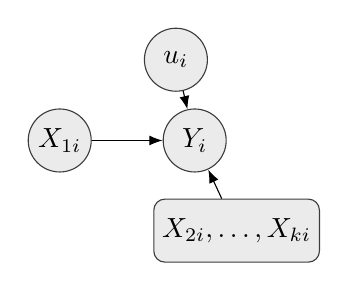
\begin{tikzpicture}[node distance=0.45cm and 0.9cm]
    \node[state] (x) at (0,0) {$X_{1i}$};
    \node[state] (y) [right =of x] {$Y_i$};
    \node[state] (u) [above right =of x] {$u_i$};
    \node[control] (c) [below right =of x] {$X_{2i},\dots,X_{ki}$};
    \path (x) edge (y);
    \path (u) edge (y);
    \path (c) edge (y);
    %\path[bidirected] (x) edge[bend right=10] (c);
  \end{tikzpicture}}
  \end{column}
  \end{columns}
  \medskip
  \pause
  \begin{block}{}
    \begin{itemize}
      \item Correlation: a statistical \textbf{measure} describing the relation between treatment $X_{1i}$ and outcome $Y_i$.
      \item Causality: a \textbf{claim} about the effect of $X_{1i}$ on $Y_i$, holding the controls and $u_i$ fixed.
      %\item[$\rightarrow$] Correlations \textbf{may} support causal claims.
    \end{itemize}
  \end{block}
\end{frame}

\section{Causality}

\begin{frame}{Potential Outcomes}
  $
    Y_i = \beta_0 + \beta_1 X_{1i} + \beta_2 X_{2i} + \dots + \beta_k X_{ki} + u_i, 
    \qquad i=1,\dots,N
    \qquad X_{1i} \in \{0,1\}
  $
  \begin{itemize}
    \item $Y_i(0) = \beta_0 + \beta_1 \cdot 0 + \beta_2 X_{2i} + \dots + \beta_k X_{ki} + u_i$: outcome of $i$ without treatment.
    \item $Y_i(1) = \beta_0 + \beta_1 \cdot 1 + \beta_2 X_{2i} + \dots + \beta_k X_{ki} + u_i$: outcome of $i$ with treatment.
  \end{itemize}
  \pause
  \vspace{0.1cm}
  Each observation belongs to either the treated or control group and has two \textbf{potential outcomes}:
  \begin{center}
    \begin{tabular}{@{}lcc@{}}
      \toprule
      & $X_{1i}=1$ (treated) & $X_{1i}=0$ (control) \\
      \midrule
      %Potential outcomes & $Y_i(1)$, $Y_i(0)$ & $Y_i(1)$, $Y_i(0)$ \\
      Observed outcome  & $Y_i=Y_i(1)$ & $Y_i=Y_i(0)$ \\
      \textcolor{red!70!black}{Missing counterfactual} & \textcolor{red!70!black}{$Y_i(0)$} & \textcolor{red!70!black}{$Y_i(1)$} \\
      \bottomrule
    \end{tabular}
  \end{center}
  \vspace{0.4cm}
  Causal effect of $X_{1i}$ on \textbf{individual} unit $i$: \quad $Y_i(1) - Y_i(0)$
   $\quad \rightarrow \quad$
    Cannot be computed.
\end{frame}

\begin{frame}{From Individual Effects to Group Comparisons}
\linespread{1.2}\selectfont
  \begin{block}{Average Treatment Effect, ATE}
    Compares mean outcomes of treated and controled units with same controls $\boldsymbol{X}_i = (X_{2i},\dots,X_{ki})$:
  \[
    ATE =
    \underbrace{\E[Y_i(1)\mid X_{1i}=1, \boldsymbol{X}_i]}_{\text{Treated}} - \underbrace{\E[Y_i(0)\mid X_{1i}=0, \boldsymbol{X}_i]}_{\text{Control}}
  \]
  \end{block}
  Adding and subtracting the treated group's \textcolor{red!70!black}{missing counterfactual}...
  \begin{align*}
    ATE&= \E[Y_i(1)\mid X_{1i}=1, \boldsymbol{X}_i] \textcolor{red!70!black}{{}- \E[Y_i(0)\mid X_{1i}=1, \boldsymbol{X}_i] + \E[Y_i(0)\mid X_{1i}=1, \boldsymbol{X}_i]{}}
    - \E[Y_i(0)\mid X_{1i}=0, \boldsymbol{X}_i]\\
    &= {\underbrace{\E[Y_i(1)-Y_i(0)\mid X_{1i}=1, \boldsymbol{X}_i]}_{\text{causal effect (on the treated)}}} +\underbrace{\E[Y_i(0)\mid X_{1i}=1, \boldsymbol{X}_i]-\E[Y_i(0)\mid X_{1i}=0, \boldsymbol{X}_i]}_{\text{selection bias}}
  \end{align*}
  \vspace{-0.2cm}
  \begin{block}{Selection Bias}
    How the treated and control group outcomes would differ \emph{even without treatment}.
  \end{block}
\end{frame}

\begin{frame}{Bringing MLR and ATE Together}
  Plugging in the regression model:
  $Y_i(X_{1i}) = \beta_0 + \beta_1 \cdot X_{1i} + \beta_2 X_{2i} + \dots + \beta_k X_{ki} + u_i \qquad X_{1i} \in \{0,1\} $
  \vspace{-0.1cm}

  
  \begin{enumerate}
    \item The causal effect simplifies to:
      $\E[Y_i(1)-Y_i(0)\mid X_{1i}=1, \boldsymbol{X}_i] = \beta_1$
    \item The selection bias $\E[Y_i(0)\mid X_{1i}=1, \boldsymbol{X}_i]-\E[Y_i(0)\mid X_{1i}=0, \boldsymbol{X}_i]$ splits into:
    \begin{itemize}
      \item differences in controls: $\sum_{j=2}^{k} \beta_j \big(\E[X_{ji}\mid X_{1i}=1, \boldsymbol{X}_i]-\E[X_{ji}\mid X_{1i}=0, \boldsymbol{X}_i]\big) 
      =
      \sum_{j=2}^{k} \beta_j \big(X_{ji} - X_{ji}\big)
      = 0$
      \item differences in unobservables: $\E[u_i\mid X_{1i}=1, \boldsymbol{X}_i]-\E[u_i\mid X_{1i}=0, \boldsymbol{X}_i]$
    \end{itemize}
  \end{enumerate}
  \pause
  ATE in a Multiple Linear Regression Model with Binary Treatment becomes:
    \[
    \textcolor{green!50!black}{ATE} = \textcolor{red!70!black}{\beta_1} + \textcolor{red!70!black}{\underbrace{\E[u_i\mid X_{1i}=1, \boldsymbol{X}_i]-\E[u_i\mid X_{1i}=0, \boldsymbol{X}_i]}_{\text{selection bias}}}
    \]
  \vspace{-0.5cm}
  \begin{center}
    When does \textcolor{green!50!black}{observed ATE} represent true \textcolor{red!70!black}{unobserved causal effect $\beta_1$}? 
    \\ 
    When does \textcolor{green!50!black}{observed ATE} also include \textcolor{red!70!black}{unobserved selection bias}?
  \end{center}
\end{frame}

\begin{comment}
  \begin{frame}{Causal Parameters (Estimands)}

  $$\tau_i = Y_i(1) - Y_i(0) = \beta_1 + u_{i(1)} - u_{i(0)}$$

  Since $\tau_i$ is unobservable, we target averages:
  \medskip
  \begin{tabular}{@{}lll@{}}
    \toprule
    Estimand & Definition & Question answered \\
    \midrule
    ATE  & $\E[Y_i(1)-Y_i(0)]$ & Random unit in the population \\
    ATT  & $\E[Y_i(1)-Y_i(0)\mid X_{1i}=1]$ & Units actually treated \\
    LATE & $\E[Y_i(1)-Y_i(0)\mid \text{complier}]$ & Units whose treatment the instrument moves \\
    \bottomrule
  \end{tabular}
  \medskip

  \begin{itemize}
    \item If effects are homogeneous ($\tau_i=\tau$ for all $i$), all three coincide. In the linear model, $\beta_1=\tau$ imposes exactly this.
    \item With heterogeneous effects, \textbf{different designs identify different estimands}. Always ask: effect \emph{for whom}?
  \end{itemize}
\end{frame}
\end{comment}

% one small causal diagram per selection-bias scenario; #1 = what links X_1i and u_i
\newcommand{\sbdag}[1]{%
  \begin{tikzpicture}[font=\scriptsize, state/.append style={minimum size=6mm}]
    % controls are held fixed in every scenario, so they are left out here
    \node[state] (x) at (0,0) {$X_{1i}$};
    \node[state] (y) at (2,0) {$Y_i$};
    \node[state] (u) at (1,0.75) {$u_i$};
    \path (x) edge (y);
    \path (u) edge node[red] {$+$} (y); % u_i enters Y_i with coefficient 1
    #1
  \end{tikzpicture}}

\begin{frame}{Average Treatment Effect and Selection Bias}
  \begin{block}{Selection Bias in MLR with Binary Treatment}
    \[
    \E[u_i\mid X_{1i}=1, \boldsymbol{X}_i]-\E[u_i\mid X_{1i}=0, \boldsymbol{X}_i]
    =
    \frac{\Cov(X_{1i},u_i\mid\boldsymbol{X}_i)}{\Var(X_{1i}\mid\boldsymbol{X}_i)}
    \]
  \end{block}
  \vspace{0.7cm}
  \begin{columns}[c]
  \begin{column}{0.7\textwidth}
  \begin{itemize}\setlength{\itemsep}{0.8em}
    \item<1-> \textbf{No bias}: $\mathrm{\Cov}(X_{1i},u_i\mid\boldsymbol{X}_i)=0 \rightarrow \text{observed } ATE= \text{unobserved } \beta_1$.
    \item<2-> \textbf{$+$ bias}: $\mathrm{\Cov}(X_{1i},u_i\mid\boldsymbol{X}_i)>0 \rightarrow \text{observed } ATE> \text{unobserved } \beta_1$.
    \item<3-> \textbf{$-$ bias}: $\mathrm{\Cov}(X_{1i},u_i\mid\boldsymbol{X}_i)<0 \rightarrow \text{observed } ATE< \text{unobserved } \beta_1$.
  \end{itemize}
  \end{column}
  \begin{column}{0.26\textwidth}
  \centering
  \only<1>{\sbdag{}}%
  \only<2>{\sbdag{\path[bidirected] (x) edge[bend left=10] node[red] {$+$} (u);}}%
  \only<3->{\sbdag{\path[bidirected] (x) edge[bend left=10] node[red] {$-$} (u);}}
  \end{column}
  \end{columns}
  \vspace{0.5cm}
  \uncover<4->{
    \begin{center}
      Causal inference's purpose: \textbf{get rid of} selection bias.
    \end{center}
  }
\end{frame}

\begin{frame}{Randomized Control Trials (RTCs)}
  \begin{columns}[c]
  \begin{column}{0.7\textwidth}
  Treatment $X_i$ is randomly assigned through a lottery.
  \begin{itemize}
    \item Mean outcomes of treated and control groups are compared.
    \item[$\rightarrow$] Unobserved ($u_i$) does not determine $X_{1i}$ assignment.
    \[
    Cov(X_{1i},u_i\mid\boldsymbol{X}_i) = 0 \quad\rightarrow\quad \text{observed } ATE = \text{unobserved } \beta_1
    \]
    \item RCT-s are the benchmark ``gold standard'' for causal inference.
  \end{itemize}
  \end{column}
  \begin{column}{0.25\textwidth}
  \centering
  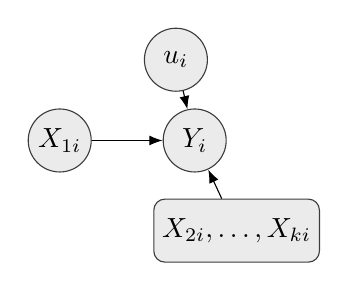
\begin{tikzpicture}[node distance=0.45cm and 0.9cm]
    \node[state] (x) at (0,0) {$X_{1i}$};
    \node[state] (y) [right =of x] {$Y_i$};
    \node[state] (u) [above right =of x] {$u_i$};
    \node[control] (c) [below right =of x] {$X_{2i},\dots,X_{ki}$};
    \path (x) edge (y);
    \path (u) edge (y);
    \path (c) edge (y);
  \end{tikzpicture}\\[0.3em]
  \end{column}
  \end{columns}
  \pause
  \vspace{0.5cm}
  Examples of RCT-s in economics:
  \begin{itemize}\setlength{\itemsep}{0pt}
    \item Free malaria \textbf{bednets} does not cause a drop in usage.
    \item School-based \textbf{deworming} treatment in Kenya caused a raise in attendance.
  \end{itemize}
\end{frame}

\begin{frame}{Limitations of RCTs}
  \begin{itemize}
    \item \textbf{Cost:} experiments are expensive and slow to run.
    \item \textbf{Feasibility:} many treatments cannot be randomized (e.g.\ taxes, minimum wages).
    \item \textbf{External validity:} results from one specific context may not generalize.
    \item \textbf{Equilibrium Effects:} treatment of one unit may affect aggregate outcomes.
    \item \textbf{Ethics:} withholding a beneficial treatment (e.g.\ bednets) from the control group.
  \end{itemize}
  \pause
  \textbf{Observational data:} Economic ``treatments'' are \textbf{not} purposefully randomized.
  \begin{itemize}
    \item[$\rightarrow$] \textbf{Next:} Minimize selection bias adding control variables.
    %\item[$\rightarrow$] The \textbf{credibility} of the causal claim dependes on \textbf{untestable} assumptions. 
  \end{itemize}
\end{frame}

\begin{frame}{The Conditional Mean Independence Assumption}
\linespread{1.1}\selectfont
  \[
    Y_i = \beta_0 + \beta_1 X_{1i} + \beta_2 X_{2i} + \dots + \beta_k X_{ki} + u_i
    \qquad
    ATE = \beta_1 + \E[u_i\mid X_{1i}=1, \boldsymbol{X}_i]-\E[u_i\mid X_{1i}=0, \boldsymbol{X}_i]
  \]
  \textbf{Selection on observables assumption:} Treatment depends on observed controls.
  \begin{itemize}
    \item Treatment is not randomly assigned\dots
    \item \dots but assigned only depends on observables.
  \end{itemize}
  \begin{block}{Selection on Observables}
    \vspace{-0.2cm}
  \begin{center}
  \resizebox{\linewidth}{!}{$
    \big(Y_i(1),Y_i(0)\big)\indep X_{1i} \mid \boldsymbol{X}_i
    \quad\rightarrow\quad
    \E[u_i \mid X_{1i}, \boldsymbol{X}_i] = \E[u_i \mid \boldsymbol{X}_i]
    \quad\rightarrow\quad
    \Cov(X_{1i},u_i\mid\boldsymbol{X}_i)=0
    \quad\rightarrow\quad
    ATE = \beta_1
  $}
  \end{center}
  \end{block}

  \begin{itemize}
    \item ATE representes the causal effect \emph{only if} this assumption holds, 
    \item It is impossible to test the assumption.
    \item Next: how to estimate $ATE$ using data?
  \end{itemize}
\end{frame}

\begin{comment}
  \begin{frame}{What Variation Identifies $\hat\beta_1$? Frisch--Waugh}
\linespread{1.2}\selectfont
  \[
    Y_i = \beta_0 + \beta_1 X_{1i} + \bm{X}_{2i}'\bm\beta_2 + u_i
  \]
  \begin{enumerate}
    \item Regress $X_{1i}$ on $\bm X_{2i}$, keep residuals $\tilde X_{1i}$
    \item Regress $Y_i$ on $\bm X_{2i}$, keep residuals $\tilde Y_i$
    \item Regress $\tilde Y_i$ on $\tilde X_{1i}$ $\Rightarrow$ slope $=\hat\beta_1$ from the full MLR
  \end{enumerate}
  \medskip
  \begin{itemize}
    \item $\hat\beta_1$ uses only the variation in $X_1$ that the controls do \emph{not} explain.
    \item \textbf{Bridge:} panel fixed effects are Frisch--Waugh with unit dummies as $\bm X_2$. Partialling out the dummies is the same as demeaning each unit's data (the ``within'' transformation).
  \end{itemize}
\end{frame}

\begin{frame}{Interpreting Coefficients: The Building Blocks}
\linespread{1.2}\selectfont
  \textbf{Dummies and interactions}
  \[
    Y_i = \beta_0 + \beta_1 D_i + \beta_2 X_i + \beta_3 (D_i\times X_i) + u_i
  \]
  Slope of $X$: $\beta_2$ if $D_i=0$; $\beta_2+\beta_3$ if $D_i=1$. Jump at $X_i=0$: $\beta_1$.
  \medskip

  \begin{columns}[T]
    \begin{column}{0.48\textwidth}
      \textbf{Logs}\\[2pt]
      \begin{tabular}{@{}ll@{}}
        \toprule
        Model & Interpretation of $\beta$ \\
        \midrule
        level--level & $\Delta Y=\beta\,\Delta X$ \\
        level--log & $\Delta Y=(\beta/100)\,\%\Delta X$ \\
        log--level & $\%\Delta Y\approx(100\beta)\,\Delta X$ \\
        log--log & $\%\Delta Y=\beta\,\%\Delta X$ \\
        \bottomrule
      \end{tabular}
    \end{column}
    \begin{column}{0.48\textwidth}
      \textbf{Where they reappear}\\[2pt]
      \begin{itemize}
        \item DiD: $\text{Treat}_i\times\text{Post}_t$
        \item Panel FE: one dummy per unit
        \item RDD: cutoff dummy $\times$ running variable
        \item Event study: one dummy per period relative to treatment
        \item Log outcomes $\Rightarrow$ effects in \%
      \end{itemize}
    \end{column}
  \end{columns}
\end{frame}
\end{comment}

\section{The OLS Estimator}

\begin{frame}{Parameters, Estimates, and Estimators}

So far, MLR featured on \textbf{population} parameters $\beta$.
We only observe a $n<N$ iid sample of the population.
\pause
\[
\underbrace{
\underset{\text{\textcolor{red!70!black}{Parameter}}}{\textcolor{red!70!black}{\beta}} 
  \xrightarrow{\text{determines}} \substack{\text{Population}}}_{\text{Unobserved}}
  %
  \xrightarrow{\text{iid draws}} 
  %
  \underbrace{\substack{\text{Dataset}}
  \xrightarrow{\text{\textcolor{red!70!black}{estimator (OLS)}}} 
  \underset{\text{\textcolor{red!70!black}{Estimate}}}{\textcolor{red!70!black}{\hat{\beta}}}}_{\text{Observed}}
\]
\pause
\begin{itemize}
    \item \textcolor{red!70!black}{Parameter ($\beta$)} is an unknown, \textbf{deterministic number} that describes relationships between two variables in the population.
    \item \textcolor{red!70!black}{Estimate ($b, \hat{\beta}$)} is a \textbf{random variable} that approximates the true parameter.
    \item \textcolor{red!70!black}{Estimator (OLS)} is a \textbf{function} that takes the data and returns an estimate.
\end{itemize}
\end{frame}

\begin{frame}{From Population to Data}
Statistical model for the unobserved \textcolor{red!70!black}{population}:
\begin{itemize}
    \item Outcome, regressors are \textbf{random variables} with joint distribution $(Y, X_1, …, X_k)$. 
    \item There is a population of size \textcolor{red!70!black}{$N$} we (almost) never get to fully observe.
    \item Error term $u_i$
    \begin{align*}
    Y_i = \textcolor{green!50!black}{\beta_0} + \textcolor{green!50!black}{\beta_1} X_{1i} + \textcolor{green!50!black}{\beta_2} X_{2i} + \cdots + \textcolor{green!50!black}{\beta_k} X_{ki} + u_i \quad i = 1, ..., \textcolor{red!70!black}{N}
    \end{align*}
\end{itemize}
\pause
Statistical model for the observed \textcolor{red!70!black}{data}:
\begin{itemize}
    \item We observe $\textcolor{red!70!black}{n} < N$ iid draws from the joint distribution.
    \item \textcolor{red!70!black}{Dataset} with $n$ observations (rows) and $k+1$ variables (columns):
    \item Residual $\hat{u}_i$
    %$$\{Y_i, X_{1i}, …,X_{ki}\}_{i = 1}^n$$
    \begin{align*}
    Y_i = \textcolor{green!50!black}{b_0} + \textcolor{green!50!black}{b_1 }X_{1i} + \textcolor{green!50!black}{b_2} X_{2i} + \cdots + \textcolor{green!50!black}{b_k} X_{ki} + \hat{u}_i \quad i = 1, ..., \textcolor{red!70!black}{n}
    \end{align*}
\end{itemize}

\end{frame}


\begin{frame}[fragile]{Writing the MLR model with vector and matrix notation}
    \begin{enumerate}
        \item A dataset with $n$ observations and $k$ covariates can be divided into:
        \begin{enumerate}
            \item $\underset{(n \times 1)}{\textbf{Y}}$ vector for grouping the outcome variable of all observations.  
            \item $\underset{(n \times k\textcolor{green!50!black}{+1})}{\textbf{X}}$ matrix grouping all the covariates and \textcolor{green!50!black}{constant term}, for all observations.
        \end{enumerate}
        \pause
        \item $\underset{(k\textcolor{green!50!black}{+1} \times 1)}{\textbf{b}}$ vector of parameter \textbf{estimates}, \textcolor{green!50!black}{including constant term $b_0$}.
        \pause
        \item $\underset{(n \times 1)}{\hat{\mathbf{u}}}$ vector stacking the residuals for all observations.
    \end{enumerate}
    \pause
    As a result, our MLR model for observed data is equivalent to a \textbf{sample} model:
    \begin{align*}
    Y_i = b_0 + b_1 X_{1i} + b_2 X_{2i} + \cdots + b_k X_{ki} + \hat{u}_i \quad \rightarrow \quad
    \textbf{Y} = \textbf{X} \times \textbf{b} + \hat{\mathbf{u}}
    \end{align*}
\end{frame}

\begin{frame}{The OLS Estimator}
\textbf{How can we estimate $\boldsymbol{\beta}$?}
\\
\pause
\begin{enumerate}
    \item Start with vector of candidate parameter estimates $\underset{(k \times 1)}{\textbf{b}}$
    \pause
    \item Compute the vector of \textbf{residuals}: 
    $$
    \underset{(n \times 1)}{\hat{\mathbf{u}}} = \underset{(n \times 1)}{\textbf{Y}} - \underset{(n \times k)}{\textbf{X}} ' \times \underset{(k \times 1)}{\textbf{b}}
    $$ \pause
    \item \textbf{Sum of Squared Residuals (SSR):} measures the overall discrepancy between the observed and predicted outcome variable:
    $$
    \underset{(1 \times 1)}{SSR(b)} = \underset{(1 \times n)}{\hat{\mathbf{u}}} ' \times \underset{(n \times 1)}{\hat{\mathbf{u}}}
    $$ \pause
    \item The Ordinary Least Squares (OLS) estimator Finds the vector of parameters $b$ that minimize $SSR(b)$. How?
\end{enumerate}
\end{frame}


\begin{frame}{OLS Estimator Formula}
Rewrite the SSR(b) objective function:
\begin{align*}
SSR(b) &= \hat{\mathbf{u}}'\hat{\mathbf{u}} \\
&=(\mathbf{Y}-\mathbf{X}\boldsymbol{b})'(\mathbf{Y}-\mathbf{X}\boldsymbol{b})\\
        &= \mathbf{Y}'\mathbf{Y}-\boldsymbol{b}'\mathbf{X}'\mathbf{Y}-\mathbf{Y}'\mathbf{X}\boldsymbol{b}+\boldsymbol{b}'\mathbf{X}'\mathbf{X}\boldsymbol{b}\\
        &=
        \mathbf{Y}'\mathbf{Y}-2\boldsymbol{b}'\mathbf{X}'\mathbf{Y}+\boldsymbol{b}'\mathbf{X}'\mathbf{X}\boldsymbol{b}
\end{align*}
\pause
To find the minimum, first-order condition with respect to vector $\boldsymbol{b}$:
\begin{align*}
\frac{\partial(\hat{\mathbf{u}}'\hat{\mathbf{u}})}{\partial\boldsymbol{b}}=-2\mathbf{X}'\mathbf{Y}+2(\mathbf{X}'\mathbf{X})\boldsymbol{b}=0
\end{align*}


Solving the first-order condition for $\mathbf{b}$ yields the OLS estimator: 
\begin{align*}
    \hat{\boldsymbol{\beta}} =
    (\mathbf{X}'\mathbf{X})^{-1}\mathbf{X}'\mathbf{Y}
\end{align*}
\end{frame}

\section{Inference}

\begin{frame}{Sampling Distribution of $\hat\beta$}
\linespread{1.2}\selectfont
  The \textbf{estimator} $\hat\beta$ is a random variable: each sample gives a different \textbf{estimate}.
  \medskip

  \begin{itemize}
    \item \textbf{Unbiased:} $\E[\hat\beta]=\beta$ (holds in any sample size)
    \item \textbf{Consistent:} $\hat\beta\xrightarrow{p}\beta$ as $n\to\infty$
    \item \textbf{Asymptotically normal:} $\hat\beta \overset{a}{\sim} N\!\left(\beta,\ \Var(\hat\beta\mid\bm X)\right)$
  \end{itemize}
  \medskip
  OLS has all three under MLR.1--MLR.4:
  \begin{itemize}
    \item \textbf{MLR.1 (Linearity):} $Y_i=\beta_0+\beta_1X_{1i}+\dots+\beta_kX_{ki}+u_i$
    \item \textbf{MLR.2 (No perfect collinearity):} no regressor is an exact linear combination of the others
    \item \textbf{MLR.3 (Random sampling):} $\{Y_i,X_{1i},\dots,X_{ki}\}_{i=1}^n$ are iid draws from the population
    \item \textbf{MLR.4 (Exogeneity):} $\E[u_i\mid X_{1i},\dots,X_{ki}]=0$
  \end{itemize}
\end{frame}

\begin{frame}{The Sandwich and Robust Standard Errors}
  \vspace{-0.2cm}
  \[
    \Var(\hat{\bm\beta}\mid\bm X) = (\bm X'\bm X)^{-1}\;\bm X'\,\E[\bm u\bm u'\mid\bm X]\,\bm X\;(\bm X'\bm X)^{-1}
  \]
  \begin{columns}[c]
  \begin{column}{0.75\textwidth}
  Everything depends on the middle term, $\bm\Omega=\E[\bm u\bm u'\mid\bm X]$:
  \medskip
  \begin{itemize}\setlength{\itemsep}{0.3em}
    \item<1-> \textbf{Homoskedastic:} same variance $\sigma^2_u$ for all errors; no correlation across observations.
    \item<2-> \textbf{Heteroskedastic robust:} each error has its own variance $\sigma^2_i$; still no correlation.
    \item<3-> \textbf{Clustered:} errors correlated within a cluster (e.g.\ school), uncorrelated across clusters.
  \end{itemize}
  \end{column}
  \begin{column}{0.25\textwidth}
  \centering
  \begin{tikzpicture}[x=0.4cm,y=0.4cm,-]
    % Homoskedastic: same variance on the diagonal, zeros elsewhere
    \only<1>{\begin{scope}
      \foreach \i in {1,...,6} \fill[red!70!black!55] (\i-1,-\i) rectangle (\i,-\i+1);
      \draw[step=1,PelloGray!40,very thin] (0,-6) grid (6,0);
      \draw[PelloGrayDark] (0,-6) rectangle (6,0);
      \node[below,font=\footnotesize,align=center,inner sep=3pt] at (3,-6) {Homoskedastic};
    \end{scope}}
    % Heteroskedastic: different variances on the diagonal, zeros elsewhere
    \only<2>{\begin{scope}
      \foreach \i/\s in {1/25,2/80,3/45,4/95,5/35,6/65}
        \fill[red!70!black!\s] (\i-1,-\i) rectangle (\i,-\i+1);
      \draw[step=1,PelloGray!40,very thin] (0,-6) grid (6,0);
      \draw[PelloGrayDark] (0,-6) rectangle (6,0);
      \node[below,font=\footnotesize,align=center,inner sep=3pt] at (3,-6) {Heteroskedastic robust};
    \end{scope}}
    % Clustered: nonzero covariances within clusters, zeros across clusters
    \only<3->{\begin{scope}
      \foreach \b in {0,2,4} \fill[red!70!black!20] (\b,-\b-2) rectangle (\b+2,-\b);
      \foreach \i/\s in {1/25,2/80,3/45,4/95,5/35,6/65}
        \fill[red!70!black!\s] (\i-1,-\i) rectangle (\i,-\i+1);
      \draw[step=1,PelloGray!40,very thin] (0,-6) grid (6,0);
      \foreach \b in {0,2,4} \draw[PelloGrayDark,thick] (\b,-\b-2) rectangle (\b+2,-\b);
      \draw[PelloGrayDark] (0,-6) rectangle (6,0);
      \node[below,font=\footnotesize,align=center,inner sep=3pt] at (3,-6) {Clustered};
    \end{scope}}
  \end{tikzpicture}\\[0.2em]
  {\tiny White $=0$; darker $=$ larger (co)variance.}
  \end{column}
  \end{columns}
\end{frame}

\begin{frame}[fragile]{Homoskedastic Standard Errors}
\linespread{1.2}\selectfont
  Assume all errors have the same variance and are uncorrelated: $\bm\Omega=\sigma^2_u\bm I_n$. The sandwich collapses to
  \[
    \Var(\hat{\bm\beta}\mid\bm X)=\sigma^2_u(\bm X'\bm X)^{-1},
    \qquad
    \hat\sigma^2_u=\frac{1}{n-k-1}\sum_{i=1}^n\hat u_i^2
  \]
  \textbf{Variance drivers} for a single coefficient:
  \[
    \Var(\hat\beta_j\mid\bm X)=\frac{1}{n}\cdot\frac{\sigma_u^2}{\sigma^2_{X_j}}\cdot\frac{1}{1-R_j^2}
  \]
  More data, less noise, more variation in $X_j$ and less collinearity ($R_j^2$) $\rightarrow$ smaller SEs.
  \begin{itemize}
    \item Default in most software, but rarely credible: the variance of $u_i$ usually depends on $X_i$.
  \end{itemize}
  \begin{lstlisting}
feols(y ~ x, data = df, vcov = "iid")
  \end{lstlisting}
\end{frame}

\begin{frame}[fragile]{Heteroskedasticity-Robust Standard Errors}
\linespread{1.2}\selectfont
  Allow each error its own variance, still uncorrelated: $\bm\Omega=\mathrm{diag}(\sigma^2_1,\dots,\sigma^2_n)$.
  \[
    \widehat{\Var}_{HC}(\hat{\bm\beta})=(\bm X'\bm X)^{-1}\Big(\sum_{i=1}^{n}\hat u_i^2\,\bm x_i\bm x_i'\Big)(\bm X'\bm X)^{-1}
  \]
  Each unknown $\sigma^2_i$ is replaced by the squared residual $\hat u_i^2$ (White, 1980).\\
  (in practice multiplied by a small-sample correction $\frac{n}{n-k-1}$, ``HC1'')
  \medskip

  \textbf{Practical rules}
  \begin{itemize}
    \item Default for cross-sectional data: valid whether or not errors are homoskedastic.
    \item Robust SEs can be larger or smaller than homoskedastic ones.
    \item They do \emph{not} fix correlation across observations $\rightarrow$ clustering.
  \end{itemize}
  \begin{lstlisting}
feols(y ~ x, data = df, vcov = "hetero")
  \end{lstlisting}
\end{frame}

\begin{frame}{Clustered Standard Errors: Why}
\linespread{1.2}\selectfont
  MLR.3 (random sampling) implies $\E[u_iu_j\mid\bm X]=0$ for $i\neq j$. This fails when observations share shocks:
  \begin{itemize}
    \item Students in the same school; firms in the same region
    \item The same unit observed over time (panel): serially correlated $u_{it}$
    \item Treatment assigned at group level (a policy in some states)
  \end{itemize}
  \medskip
  \textbf{Moulton factor} (equal-sized groups of size $\bar n$):
  \[
    \frac{\Var_{\text{true}}(\hat\beta)}{\Var_{\text{iid}}(\hat\beta)} \approx 1 + (\bar n-1)\,\rho_X\,\rho_u
  \]
  $\rho_X,\rho_u$: within-cluster correlation of regressor and error. If $X$ is constant within clusters ($\rho_X=1$) and groups are large, iid SEs can be wildly too small.
\end{frame}

\begin{frame}[fragile]{Clustered Standard Errors: How}
\linespread{1.2}\selectfont
  Allow arbitrary correlation \emph{within} clusters $g=1,\dots,G$, independence \emph{across} them:
  \[
    \widehat{\Var}_{CL}(\hat{\bm\beta})=(\bm X'\bm X)^{-1}\Big(\sum_{g=1}^{G}\bm X_g'\,\hat{\bm u}_g\hat{\bm u}_g'\,\bm X_g\Big)(\bm X'\bm X)^{-1}
  \]
  (in practice multiplied by a small-sample correction $\frac{G}{G-1}\frac{n-1}{n-k-1}$)
  \medskip

  \textbf{Practical rules}
  \begin{itemize}
    \item Cluster at the level at which treatment is assigned (Abadie et al., 2023).
    \item Panel/DiD: cluster by unit to allow serial correlation (Bertrand, Duflo \& Mullainathan, 2004).
    \item Asymptotics are in $G$, not $n$: with few clusters ($G\lesssim 30$--$50$) use the wild cluster bootstrap.
  \end{itemize}
  \begin{lstlisting}
library(fixest)
feols(y ~ x | unit + year, data = df, cluster = ~unit)
  \end{lstlisting}
\end{frame}

\begin{frame}{Tests and Confidence Intervals: Correct Interpretation}
\linespread{1.2}\selectfont
  $t$-statistic: $T=\dfrac{\hat\beta_j-\beta_{j,0}}{\SEhat(\hat\beta_j)}\overset{a}{\sim}N(0,1)$ under $H_0$. Reject at level $\alpha$ if $|T|>z_{1-\alpha/2}$.
  \medskip

  \begin{itemize}
    \item \textbf{p-value:} the probability, \emph{if $H_0$ were true}, of a test statistic at least as extreme as the one observed.\\ It is \textbf{not} the probability that $H_0$ is true.
    \item \textbf{95\% CI} $[\hat\beta_j\pm1.96\,\SEhat(\hat\beta_j)]$: across repeated samples, 95\% of intervals constructed this way cover $\beta_j$. A given realized interval either contains $\beta_j$ or it does not.
    \item \textbf{Statistical vs.\ economic significance:} report effect sizes (e.g.\ the effect of a 1-SD change in $X_j$), not just stars.
  \end{itemize}
  \medskip
  The SEs (robust or clustered) determine everything on this slide, so choosing them is a substantive decision.
\end{frame}

\section{Conclusion}

\begin{frame}{The Limits of ``Just Add Controls''}
\linespread{1.2}\selectfont
  \begin{itemize}
    \item Adding every relevant covariate would remove the bias, but we can never verify that we have them all.
    \item Some confounders are unobservable by nature (ability, motivation, local politics).
    \item Controls do not solve measurement error or reverse causality.
    \item ``Bad controls'': controlling for a variable that is itself an outcome of treatment introduces bias.
  \end{itemize}
  \medskip
  \textbf{Modern approach:} instead of trying to observe every confounder, find a \emph{source of variation} in $X$ that is plausibly unrelated to the confounders.
  \medskip

  That source of variation is the \emph{research design}.
\end{frame}


\begin{frame}{One Map: What Each Design Assumes Instead}
\linespread{1.2}\selectfont
  \begin{tabular}{@{}llll@{}}
    \toprule
    Design & Replaces $\E[u_i\mid X_i]=0$ with & Estimand & Inference \\
    \midrule
    RCT & Random assignment & ATE & robust \\
    MLR & Selection on observables & ATE (if CIA) & robust \\
    IV & Instrument exogenous + relevant & LATE & robust / clustered \\
    Panel FE & Strict exogeneity given unit FE & within-unit effect & cluster by unit \\
    DiD & Parallel trends & ATT & cluster by unit/group \\
    RDD & Continuity at the cutoff & local effect at cutoff & robust / bias-corrected \\
    \bottomrule
  \end{tabular}
  \medskip

  \normalsize
  Each design is still a regression. What differs is \emph{which variation} identifies $\beta$, and \emph{why} that variation is credibly unrelated to $u_i$.
\end{frame}

\begin{frame}{Recap}
\linespread{1.2}\selectfont
  \begin{itemize}
    \item Causal questions come first: potential outcomes define \emph{what} we estimate (ATE, ATT, LATE).
    \item OLS estimates partial correlations. It is causal only under $\E[u_i\mid X_i]=0$, which is unverifiable with observational data.
    \item One formula diagnoses the failure: $\plim\hat\beta_1=\beta_1+\Cov(X,u)/\Var(X)$.
    \item Inference depends on $\bm\Omega$: robust SEs for cross-sections, clustered SEs whenever errors are correlated within groups.
    \item IV, FE, DiD and RDD reuse the same tools (dummies, interactions, Frisch--Waugh, the sandwich) with a different identifying assumption. The quality of a design is the credibility of that assumption.
  \end{itemize}
\end{frame}

\end{document}
